\chapter{Notes}

A Note is similar to a postit note. A Note has only two parts - name and content.
The name of a Note is the identifier used for display purposes. The name can also be used to search for a Note of interest.
The content is the textual information in the Note.
A Note can be standalone or placed inside a Container. In this section we are explaining the operations associated with a standalone Note. However, the principles outlined here applies to a Note created as an Item inside a Container too.
Notes can be Private or Shareable.
A Private Note cannot be shared with any user.

\section{Create a Note}
From the top \textbf{Notes} menu, select \textbf{Create New Note}. The resulting screen will be as in the following figure:

\begin{figure}[H]
\centering
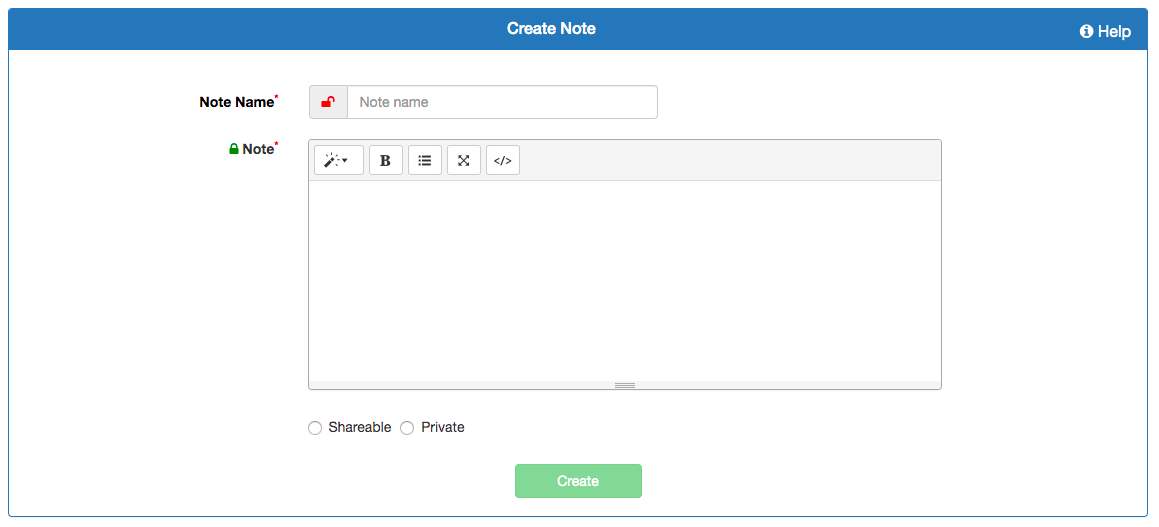
\includegraphics[scale=0.4]{user/Create-Note.png}
\caption{Create New Note}
\label{fig: Figure}
\end{figure}

When creating a Shareable Note, it is possible to set an expiration. The user can specify the date on which the Note will expire. 
Once a Note expires, it will not be accessible to the shared users/groups.
It is not possible to set expiration on a Private Note.

\section{List Notes}
Select \textbf{List My Notes} from the top level \textbf{Notes} menu.
The result with be similar to the figure shown below:

\begin{figure}[H]
\centering
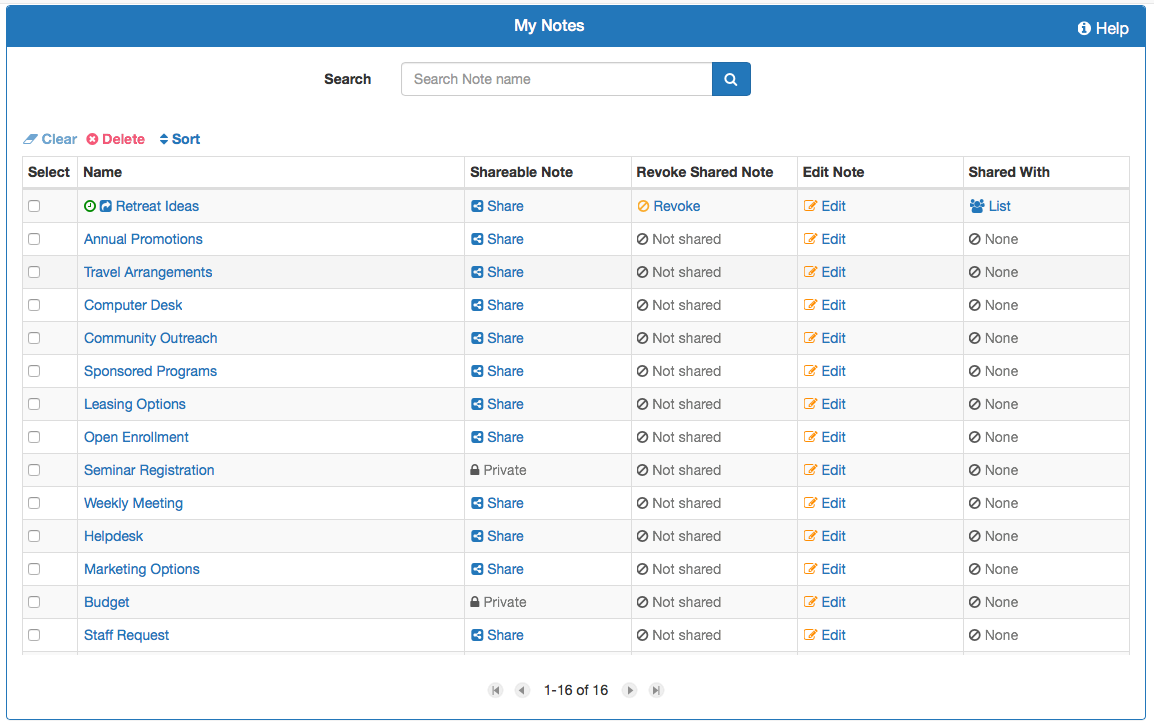
\includegraphics[scale=0.425]{user/List-My-Notes.png}
\caption{List My Notes}
\label{fig: Figure}
\end{figure}

The order of listing of Notes can be changed using the {\color{myblue}\faSort \ Sort} option.

\begin{figure}[H]
\centering
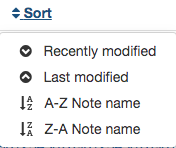
\includegraphics[scale=0.5]{user/Sort-Menu.png}
\caption{Sort Notes}
\label{fig: Figure}
\end{figure}

\section{View a Note}
Get the List of Notes (see section above). Click on the name of the Note to view it.

\begin{figure}[H]
\centering
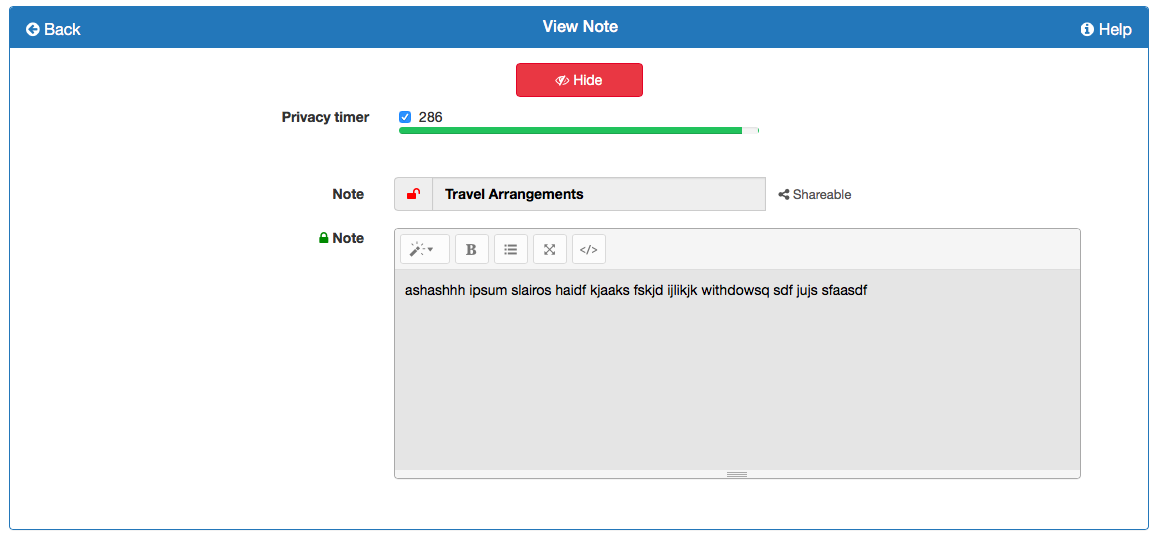
\includegraphics[scale=0.425]{user/View-Note.png}
\caption{View Note}
\label{fig: Figure}
\end{figure}

\section{Edit a Note}
From the List of Notes, a Note can be edited by clicking the {\color{orange}\faEdit} {\color{myblue}Edit} link.

\section{Delete a Note}
From the List of Notes, select the Note(s) to delete by clicking on the select button to the left of Note(s). 
Then click on {\color{red}\faTimesCircle \ Delete}. You will be asked to confirm the deletion. 

Note: When a Note is deleted, it will also be removed from all users to whom it was previously shared.

\section{Share a Note}
Sharing a Note can be done only from the List of Notes (see section above).
From the List of Notes, on the line corresponding to the Note, click on {\color{myblue}\faShareAltSquare \ Share} to initiate sharing of the Note.
